\chapter{Desenvolvimento da Proposta de Solução}
\label{chap:desenvolvimento_proposta}

O desenvolvimento do Aerochord foi pautado pelo desafio central de conciliar duas cargas computacionais de naturezas distintas: o processamento intensivo e variável de visão computacional (inferência de redes neurais) e a exigência de latência mínima e determinística para a geração de comandos musicais. Para atingir esse objetivo, a arquitetura do sistema foi projetada sob o paradigma de esteira de processamento assíncrona (\textit{pipeline}), desenvolvida em C++17 e integrando o arcabouço (\textit{framework}) JUCE para manipulação de eventos MIDI e a biblioteca MediaPipe para detecção de pose.

Este capítulo detalha a modelagem de requisitos, a arquitetura da solução e o fluxo de dados — desde a captura do movimento até a síntese do comando sonoro —, evidenciando as estratégias de engenharia de \textit{software} adotadas para garantir estabilidade e precisão em tempo real.

\section{Modelagem de Casos de Uso}
\label{sec:casos_de_uso}

Para formalizar as interações entre o usuário e o hiperinstrumento, elaborou-se o Diagrama de Casos de Uso (Figura~\ref{fig:diagrama_casos_uso}). Na modelagem, o único ator externo primário é o **Músico** (ou intérprete), que interage com o sistema exclusivamente por meio de gestos no espaço tridimensional capturados pela câmera.

\begin{figure}[htbp!]
    \caption{Diagrama de Casos de Uso do Aerochord}
    \centering 
    \label{fig:diagrama_casos_uso}
    % Nota: Salve a imagem gerada pelo PlantUML na pasta "imagens" com o nome "casos_uso.png"
    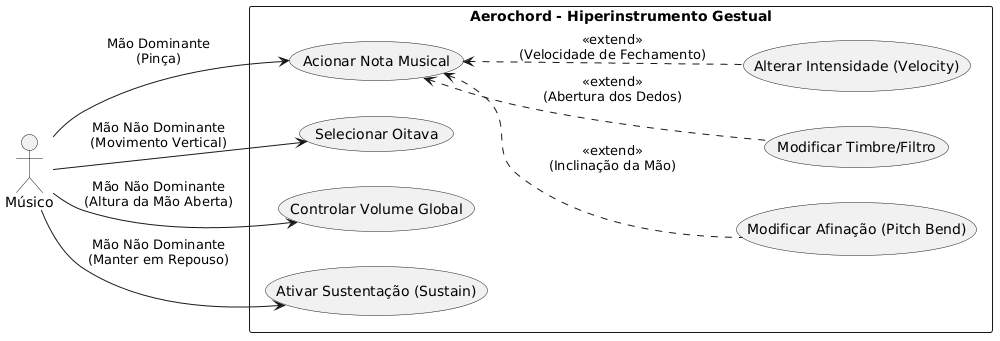
\includegraphics[width=0.85\linewidth]{imagens/casos_uso.png}
    \fonte{O Autor (2026).}
\end{figure}

O sistema prevê os seguintes casos de uso principais, que são acionados simultaneamente dependendo do papel de cada mão (controle ou articulação, atribuído por ordem de entrada em quadro — ver Seção~\ref{sec:captura_deteccao}):
\begin{itemize}
    \item \textbf{Acionar Nota:} O caso de uso central, onde o músico realiza o fechamento dos dedos para engatilhar um evento sonoro.
    \item \textbf{Modular Afinação (\textit{Pitch Bend}):} Ação contínua e simultânea à nota ativada, alterando a altura da nota através da inclinação da mão.
    \item \textbf{Controlar Timbre/Filtro:} Modulação contínua do som utilizando a abertura dos dedos.
    \item \textbf{Controlar Volume e Oitava:} Ações de macrocontrole, operadas pela mão de controle, que configuram a região tonal e a intensidade global do som.
    \item \textbf{Acionar Sustentação (\textit{Sustain}):} Manutenção do som após a liberação do gesto original.
\end{itemize}

\section{Arquitetura do Sistema e Concorrência}
\label{sec:arquitetura_concorrencia}

A arquitetura do Aerochord é composta por cinco módulos principais de processamento, além de um módulo opcional de visualização. Para evitar gargalos e garantir que a lentidão momentânea na inferência de vídeo não bloqueie a emissão de comandos MIDI, cada módulo opera em sua própria linha de execução (\textit{thread}) dedicada.

A comunicação inter-processual é realizada exclusivamente por meio de filas de produtor único e consumidor único (\textit{Single-Producer / Single-Consumer} - SPSC) do tipo livres de bloqueio (\textit{lock-free}). Esta estrutura, implementada por meio de espaços de armazenamento temporário (\textit{buffers}) circulares estáticos e operações atômicas com barreiras de memória rigorosas, elimina a necessidade de mecanismos de exclusão mútua (\textit{mutexes}). Na prática, isso impede que uma \textit{thread} bloqueie a outra (\textit{thread blocking}), garantindo que o fluxo de dados musicais no caminho crítico de execução (\textit{hot path}) ocorra sem interrupções por sincronização, requisito fundamental em sistemas de áudio de baixa latência.

O fluxo contínuo de dados atravessa os seguintes estágios:
\begin{enumerate}
    \item \textbf{Captura:} Obtenção de quadros da câmera.
    \item \textbf{Detecção de Pose:} Extração de coordenadas espaciais das mãos.
    \item \textbf{Análise de Gestos:} Tradução de coordenadas em eventos com significado semântico através de uma Máquina de Estados Finitos (\textit{Finite State Machine} - FSM).
    \item \textbf{Mapeamento:} Conversão de intenções gestuais em comandos musicais brutos.
    \item \textbf{Geração MIDI:} Empacotamento e transmissão de protocolos musicais (MIDI 1.0/2.0).
\end{enumerate}

\section{Captura e Detecção de Pose}
\label{sec:captura_deteccao}

A primeira etapa do \textit{pipeline} é gerenciada pelo módulo de captura (\texttt{CaptureModule}), responsável por interagir diretamente com o equipamento físico (\textit{hardware}) de vídeo. Em ambientes Linux, o módulo utiliza a interface V4L2 (\textit{Video4Linux2}) com mapeamento direto de memória (\textit{memory mapping}) para acessar os \textit{buffers} da câmera, evitando cópias desnecessárias na memória do sistema. 

Na sequência, o módulo de detecção (\texttt{PoseDetectionModule}) consome esses quadros e aciona o rastreador de pontos-chave das mãos (\textit{Hand Landmarker}) do MediaPipe. Este módulo extrai 21 pontos de referência anatômicos (\textit{landmarks}) tridimensionais normalizados para até duas mãos simultaneamente. Para mitigar o \textit{jitter} (pequenas oscilações naturais e ruídos na inferência da rede neural) que poderia resultar em ruído sonoro, o sistema aplica um filtro de Média Móvel Exponencial (EMA) sobre as coordenadas espaciais. Adicionalmente, um algoritmo de correspondência espacial por proximidade do pulso garante que as detecções não troquem de papel inadvertidamente entre os quadros, preservando a coerência da atribuição de cada mão ao longo do tempo.

A atribuição inicial dos papéis de cada mão (controle vs.\ articulação) é feita por \textbf{ordem de entrada em quadro}, e não pela classificação de lateralidade (esquerda/direita) do MediaPipe: a primeira mão detectada após um período sem nenhuma mão em quadro assume o papel de controle (volume/oitava); a segunda mão a entrar assume o papel de articulação (pinça/notas). Essa escolha de projeto decorre da baixa confiabilidade da classificação de lateralidade do MediaPipe quando apenas uma mão está visível, sem o contexto da outra mão para comparação — o que tornaria o rótulo bruto do modelo uma base instável para a divisão de papéis. Como efeito colateral desejável, esse critério torna o sistema utilizável tanto por destros quanto por canhotos sem qualquer configuração: o usuário simplesmente posiciona primeiro a mão que deseja usar para controle.

\section{Máquina de Estados e Análise Gestual}
\label{sec:fsm_analise}

O módulo de análise (\texttt{GestureAnalysisModule}) atua como o motor lógico do sistema. Ele ingere as coordenadas filtradas e extrai métricas geométricas, como distâncias euclidianas e ângulos relativos, alimentando a Máquina de Estados Finitos (FSM) que identifica a intenção musical do usuário.

Visando acessibilidade e ergonomia irrestrita (suportando usuários destros e canhotos sem qualquer configuração prévia), o sistema divide as responsabilidades entre dois papéis funcionais, atribuídos por ordem de entrada em quadro conforme descrito na Seção~\ref{sec:captura_deteccao}:
\begin{itemize}
    \item \textbf{Mão de Articulação e Modulação (segunda a entrar em quadro):} Controla o gatilho das notas através de um gesto de "pinça" (aproximação entre polegar e indicador). A FSM transita pelos estados de inatividade (\texttt{IDLE}), início de pinça (\texttt{PINCH\_START}) e sustentação de pinça (\texttt{PINCH\_HOLD}). Durante a sustentação, o módulo extrai variações contínuas, como o ângulo de inclinação da mão para modulação de afinação (\textit{Pitch Bend}) e a taxa de oscilação lateral para controle de \textit{Vibrato}.
    \item \textbf{Mão de Macrocontrole (primeira a entrar em quadro):} Opera majoritariamente de forma contínua. A altura vertical da mão aberta traduz-se em controle global de volume. Um gesto de pinça acompanhado de movimento vertical aciona a transição de oitavas, enquanto manter a mão em repouso por um período pré-determinado alterna o estado do pedal de sustentação (\textit{Sustain}).
\end{itemize}

Como o papel de cada mão é definido pela ordem de entrada e não pela lateralidade anatômica, o usuário escolhe livremente qual mão (esquerda ou direita) deseja usar para articulação, bastando posicioná-la em quadro depois da mão de controle.

Para garantir estabilidade, o módulo implementa lógicas de estabilização de sinal (\textit{debounce}, exigindo estabilidade por quadros consecutivos) e \textit{histerese} (diferença de limiares) nas transições de estado, prevenindo engatilhamentos duplos e acidentais das notas.

\section{Estratégias de Mapeamento Gesto-Som}
\label{sec:estrategias_mapeamento}

O módulo de mapeamento (\texttt{MappingModule}) consome os eventos gestuais semânticos e os traduz em comandos MIDI, atuando como a interface entre o movimento físico e a teoria musical.

A Tabela~\ref{tab:mapeamento_implementado} descreve o conjunto de mapeamentos implementados, detalhando cada gesto básico, a ação musical correspondente e a justificativa para a escolha do gesto em termos ergonômicos e perceptivos, respeitando a lógica de lateralidade.

\begin{table}[htbp]
    \centering
    \caption{Mapeamento Gesto–Som Implementado no Aerochord}
    \label{tab:mapeamento_implementado}
    {\scriptsize
     \setlength{\tabcolsep}{2pt}
     \renewcommand{\arraystretch}{1.0}
     \begin{tabularx}{\textwidth}{L{2.5cm} L{2cm} L{4.5cm} X}
        \toprule
        \textbf{Função Musical} & \textbf{Mão (ordem de entrada)} & \textbf{Gesto Utilizado} & \textbf{Justificativa} \\
        \midrule
        Seleção de Oitava 
            & 1\textsuperscript{a} (controle)
            & Pinça + movimento vertical. 
            & Gesto modal claro que separa o controle de oitava de outras funções, evitando acionamentos acidentais. \\
        \addlinespace
        Volume Global 
            & 1\textsuperscript{a} (controle)
            & Mão aberta + movimento vertical. 
            & Mapeamento intuitivo (cima/baixo = mais/menos) que utiliza um gesto natural de ``repouso''. \\
        \addlinespace
        Disparo de Nota 
            & 2\textsuperscript{a} (articulação)
            & Pinça (polegar + indicador) em zonas verticais discretas. 
            & Gesto ergonômico e preciso para iniciar o som. A altura da mão define a nota de forma intuitiva. \\
        \addlinespace
        Parada de Nota 
            & 2\textsuperscript{a} (articulação)
            & Soltar o gesto de pinça. 
            & Ação de abrir a mão é a contraparte mecânica e imediata ao gesto de disparo. \\
        \addlinespace
        Timbre/Filtro 
            & 2\textsuperscript{a} (articulação)
            & Distância entre a ponta do dedo médio e a palma. 
            & Gesto robusto para rastreamento que oferece grande amplitude expressiva sem influenciar a afinação. \\
        \addlinespace
        \textit{Pitch Bend} 
            & 2\textsuperscript{a} (articulação)
            & Inclinação (rotação) da mão. 
            & Movimento angular é ortogonal ao movimento de seleção de nota, minimizando conflitos de leitura. \\
        \addlinespace
        \textit{Vibrato} 
            & 2\textsuperscript{a} (articulação)
            & Oscilação leve lateral. 
            & Mimetiza mecanicamente o \textit{vibrato} de instrumentos de corda acústicos. \\
        \addlinespace
        Intensidade (\textit{Velocity}) 
            & 2\textsuperscript{a} (articulação)
            & Velocidade temporal de fechamento da pinça. 
            & Imita a física de instrumentos de percussão e teclas (tocar mais rápido gera um ataque mais intenso). \\
        \bottomrule
     \end{tabularx}
    }
\end{table}

Observa-se que a mão de controle foi minimamente utilizada, o que abre margem para expansões futuras de controle (como acionamento de acordes inteiros ou mudança de programas). O mapeamento discrimina claramente ações discretas (ativação de nota) e modulações contínuas.

O sistema divide a área de atuação da câmera em 12 zonas verticais, correspondentes aos semitons de uma oitava completa. O mapeamento incorpora zonas mortas (\textit{dead zones} — áreas de fronteira sem resposta) e preenchimento (\textit{padding}) nas extremidades superior e inferior do quadro visual. Isso fixa as notas mais graves e agudas, garantindo que o \textit{performer} não precise esticar o braço até os limites físicos do alcance da câmera para tocar as notas extremas da escala.

Um recurso de destaque na implementação é o modo de ligação (\textit{legato}). Quando ativado, o mapeador permite a transição de notas de forma fluida (deslizando a mão de articulação ainda fechada entre as zonas verticais). A engenharia do módulo garante que o comando da nova nota (\texttt{NOTE\_ON}) seja emitido milissegundos antes do encerramento da nota anterior (\texttt{NOTE\_OFF}), criando a sobreposição de áudio necessária para que os sintetizadores engatilhem transições fluídas, mimetizando instrumentos de sopro.

\section{Geração de Protocolo e Suporte Nativo a MIDI 2.0}
\label{sec:geracao_protocolo}

A etapa final reside no módulo de comunicação, responsável por formatar e entregar os comandos musicais ao sistema operacional. O Aerochord inova ao implementar suporte ao padrão MIDI 2.0 através da formatação de Pacotes MIDI Universais (\textit{Universal MIDI Packet} - UMP).

Durante a inicialização, o sistema executa um processo de negociação inicial (\textit{handshake}) via Consulta de Capacidades (\textit{Capability Inquiry} - MIDI-CI), enviando mensagens de descoberta (\textit{Discovery}) para verificar se o dispositivo receptor suporta a nova especificação. Sendo compatível, o sistema constrói pacotes UMP de 64 bits e os despacha. Isso garante resoluções de 32 bits para mensagens de controle contínuo, além de permitir o \textit{Per-Note Pitch Bend} (dobra de afinação individualizada por nota ativa), elevando drasticamente o teto de expressividade instrumental da aplicação.

Caso o equipamento ou \textit{software} receptor não suporte o novo padrão, o sistema aplica um mecanismo de contingência (\textit{fallback}) transparente, truncando matematicamente os dados para os 7 bits originais e roteando a comunicação via arquitetura legado (MIDI 1.0), assegurando total compatibilidade com tecnologias anteriores e garantindo a universalidade da solução.